The initial step of our work is the study of the existing MC TBR model and its
behaviour. Following the examination of its features (simulation parameters), we
present efficient means of evaluating this model on large sets of points in
high-performance computing (HPC) environment, preprocessing techniques designed
to adapt collected datasets for surrogate modelling, and our attempts at feature
space reduction to achieve the lowest possible number of dimensions.


\subsection{Expensive Model Description}
\label{sec:expensive-model-description}

The MC TBR model that we understand to be the expensive function for our
surrogate modelling is fundamentally a Monte Carlo simulation based on the OpenMC
framework. At input the software expects a set of 19~parameters, discrete and
continuous, that are fully listed in~\cref{tbl:params}. Following a brief period of
time (usually on the order of tens of seconds), during which a fixed number of events is simulated, the software outputs the
mean and the standard deviation of the TBR aggregated over the simulated run. The
former of these two outputs we accept to be the output TBR value that is subject
to approximation.

\begin{table}[h]
	\centering
	{\footnotesize
		\begin{tabular}{l|lllll}
		\toprule
		{} & Parameter Name & Acronym & Type & Domain & Description\\
		\midrule
		\parbox[t]{2mm}{\multirow{12}{*}{\rotatebox[origin=c]{90}{Blanket}}}
		   & Breeder fraction\textsuperscript{\textdagger} & BBF & Continuous & $[0,1]$ & TODO\\
		   & Breeder \isotope[6]{Li} enrichment fraction & BBLEF & Continuous & $[0,1]$ & {}\\
		   & Breeder material & BBM & Discrete & $\{\ce{Li2TiO3}, \ce{Li4SiO4}\}$ & {}\\
		   & Breeder packing fraction & BBPF & Continuous & $[0,1]$ & {}\\
		   & Coolant fraction\textsuperscript{\textdagger} & BCF & Continuous & $[0,1]$ & {}\\
		   & Coolant material & BCM & Discrete & $\{\ce{D2O}, \ce{H2O}, \ce{He}\}$ & {}\\
		   & Multiplier fraction\textsuperscript{\textdagger} & BMF & Continuous & $[0,1]$ & {}\\
		   & Multiplier material & BMM & Discrete & $\{\ce{Be}, \ce{Be12Ti}\}$ & {}\\
		   & Multiplier packing fraction & BMPF & Continuous & $[0,1]$ & {}\\
		   & Structural fraction\textsuperscript{\textdagger} & BSF & Continuous & $[0,1]$ & {}\\
		   & Structural material & BSM & Discrete & $\{\ce{SiC}, \text{eurofer}\}$ & {}\\
		   & Thickness & BT & Continuous & $[0,500]$ & {}\\
		\midrule
		\parbox[t]{2mm}{\multirow{7}{*}{\rotatebox[origin=c]{90}{First wall}}}
		   & Armour fraction\textsuperscript{\textdaggerdbl} & FAF & Continuous & $[0,1]$ & {}\\
		   & Armour material & FAM & Discrete & $\{\text{tungsten}\}$ & {}\\
		   & Coolant fraction\textsuperscript{\textdaggerdbl} & FCF & Continuous & $[0,1]$ & {}\\
		   & Coolant material & FCM & Discrete & $\{\ce{D2O}, \ce{H2O}, \ce{He}\}$ & {}\\
		   & Structural fraction\textsuperscript{\textdaggerdbl} & FSF & Continuous & $[0,1]$ & {}\\
		   & Structural material & FSM & Discrete & $\{\ce{SiC}, \text{eurofer}\}$ & {}\\
		   & Thickness & FT & Continuous & $[0,20]$ & {}\\
		\bottomrule
		\end{tabular}
	}
	\caption{Input parameters supplied to the MC TBR simulation in alphabetical
		order. Fractions marked with superscripts\textsuperscript{\textdagger
		\textdaggerdbl} are independently required to sum to one.}
	\label{tbl:params}
\end{table}

In our work, we often reference TBR points or samples. These are simply vectors
in the feature space generated by Cartesian product of domains of all
features---parameters from~\cref{tbl:params}.

Since most surrogate models
that we employ assume overall continuous inputs, we take steps to unify our
feature interface in order to attain this property. In particular, we eliminate
discrete features by embedding each such feature into a finite multitude of
continuous features using standard one-hot encoding. This option is available to
us since discrete domains that generate our feature space are finite in
cardinality and relatively small in size. And while it renders all features continuous, the
modification comes at the expense of increasing the dimensionality of the
feature space to 27 features in total. This is further discussed
in~\cref{sec:dimred}.


\subsection{Dataset Generation}
\label{sec:dataset-generation}

While we deliberately make no assumptions about the internal properties of the
MC TBR simulation, effectively treating it as a black box model, our means of
studying its behaviour are limited to inspection of its outputs at various
points in the feature space, and inference thereof. We thus require to
gather sufficiently large and representative quantities of samples to ensure
statistical significance of our findings.

With grid search in high-dimensional domain clearly intractable, we decided to
implement uniform pseudo-random sampling to generate large amounts of feature
configurations that we consider to be independent and unbiased. For evaluation
of the expensive MC TBR model, we utilise parallelisation offered by
the HPC infrastructure available at UCL computing facilities. To this end, we
implemented the Approximate TBR Evaluator---a Python software package capable of
sequential evaluation of the multi-threaded OpenMC simulation on batches of
previously generated points in the feature space.
We deployed ATE at the UCL Hypatia cluster RCIF partition, which consists of
4~homogeneous nodes, each containing 40 cores. We completed three data
generation runs, which are summarised in~\cref{tbl:sampling-runs}.

\begin{table}[h]
	\centering
	{\footnotesize
		\begin{tabular}{rllll}
		\toprule
		\#	& Sample count & Batch division & Run time (incl. waiting) & Description \\
		\midrule
		0 & \num{100000} & $\num{100}\times\num{1000}$ & 2~days, 23~hours &
		Testing run using older MC TBR version.\\
		1 & \num{500000} & $\num{500}\times\num{1000}$ & 13~days, 20~hours &
		Fully uniform sampling in the entire domain.\\
		2 & \num{400000} & $\num{400}\times\num{1000}$ & 10~days &
		Mixed sampling, discrete features fixed.\\
		\bottomrule
		\end{tabular}
	}
	\caption{Parameters of sampling runs.}
	\label{tbl:sampling-runs}
\end{table}

Skipping run zero, which was performed using older, fundamentally different
version of the MC TBR software, and was thus treated as a technical
proof-of-concept, we generated the total of~\num{900000} samples in two runs.
While the first run featured fully uniform sampling of the unrestricted feature
space, the second run used more elaborate strategy. Interested in further study
of relationships between discrete and continuous features, we selected four
assignments of discrete features (listed in~\cref{tbl:slices}) and fixed them
for all points, effectively slicing the feature space into four corresponding
subspaces. In order to achieve comparability between these \textit{slices}, the
remaining unassigned features were uniformly sampled only in the first slice,
and reused in the other three.

\begin{table}[h]
	\centering
	{\footnotesize
		\begin{tabular}{r|lllllll}
		\toprule
		{} & \multicolumn{7}{c}{Discrete feature assignment}\\
		Batches & BBM & BCM & BMM & BSM & FAM & FCM & FSM \\
		\midrule
		0-99 & \ce{Li4SiO4} & \ce{H2O} & \ce{Be12Ti} & eurofer & tungsten & \ce{H2O} & eurofer\\
		100-199 & \ce{Li4SiO4} & \ce{He} & \ce{Be12Ti} & eurofer & tungsten & \ce{H2O} & eurofer\\
		200-299 & \ce{Li4SiO4} & \ce{H2O} & \ce{Be12Ti} & eurofer & tungsten & \ce{He} & eurofer\\
		300-399 & \ce{Li4SiO4} & \ce{He} & \ce{Be12Ti} & eurofer & tungsten & \ce{He} & eurofer\\
		\bottomrule
		\end{tabular}
	}
	\caption{Selected discrete feature assignments corresponding to slices in run~2.}
	\label{tbl:slices}
\end{table}

Since some methods applied in this work are not scale-invariant or
perform suboptimally when presented with arbitrarily scaled problems, all results
produced in the sampling runs were standardised prior to further use. In this
commonly used statistical procedure, features and regression outputs are
independently scaled and offset to attain zero mean and unit variance.



\subsection{Dimensionality Reduction}
\label{sec:dimred}

% TODO: here maybe mention desirable effects of dim. red. (e.g. speedup,
% simplification of the problem, better convergence...)

Model training over high-dimensional parameter spaces may be facilitated by carefully reducing the number of variables used to describe the space. For many applications, feature selection strategies succeed in identifying a sufficiently representative subset of the original input variables; however, all given variables were assumed to be physically relevant to the MC TBR model. Feature extraction methods, on the other hand, aim to identify a transformation from the parameter space which decreases dimensionality; even if no individual parameter is separable from the space, some linear combinations of parameters or nonlinear functions of parameters may be.

\begin{figure}[h]
	\centering
	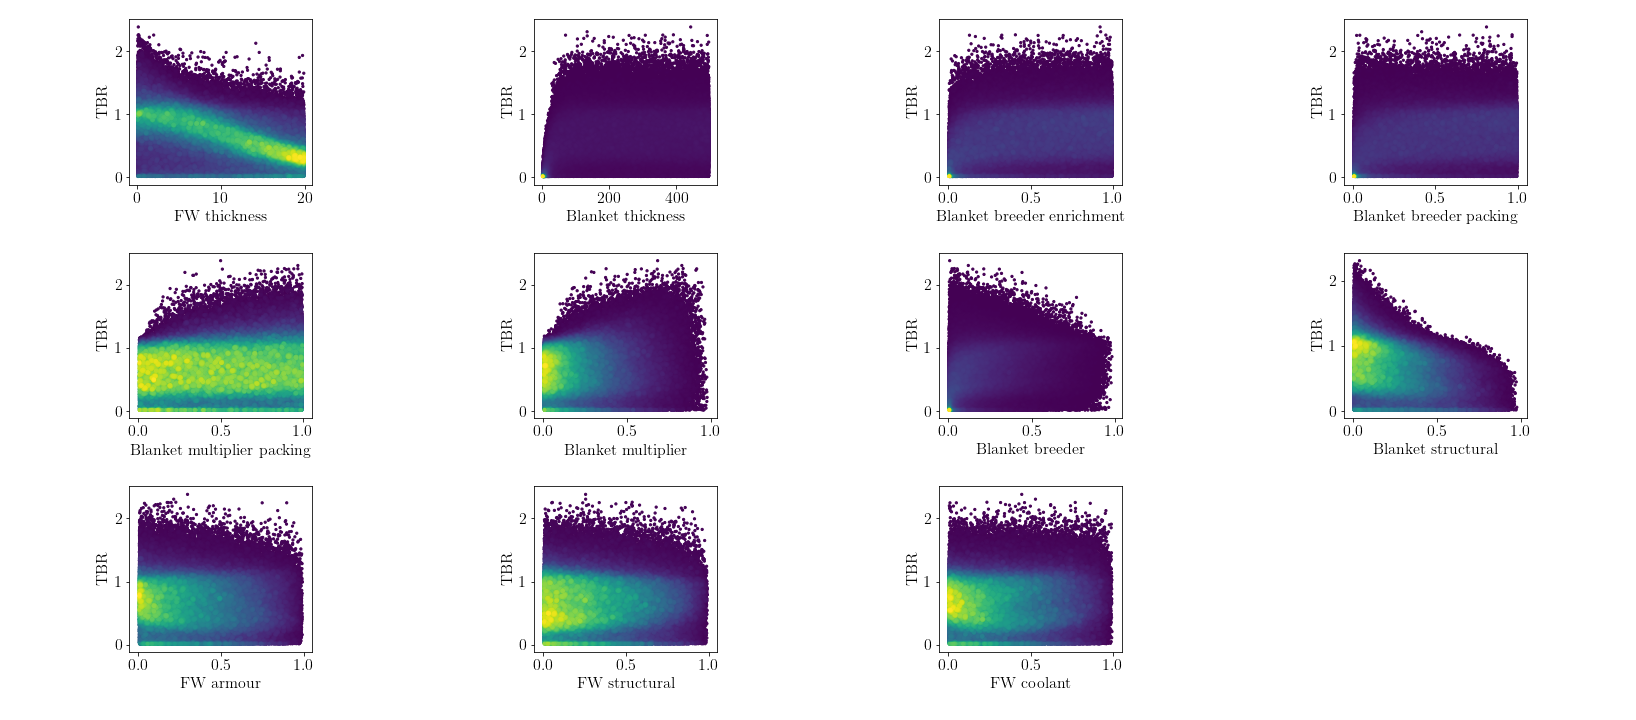
\includegraphics[width=\linewidth]{run1_400k_tbr_vs_feat}
	% TODO: placeholder only, turn into vector
	\caption{Marginalised dependence of TBR on the choice of continuous
	features.}
  \label{fig:tbr-vs-features}
\end{figure}

\subsubsection{Principal Component Analysis}

To pursue linear feature extraction, principal component analysis (PCA)
\cite{Jolliffe2016} was performed via SciKit Learn~\cite{scikit-learn} on a set
of \num{300000} uniform samples of the MC TBR model. % TODO:which run? batch range?

\Cref{fig:pca} shows the resultant cumulative variance of the feature vectors identified by PCA. The similar share of variance among all eleven features demonstrated irreducibility of the TBR model by linear methods.

\begin{figure}[h]
  \centering
    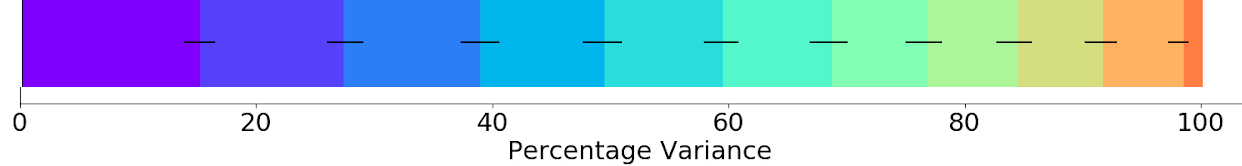
\includegraphics[width=0.6\linewidth]{fig2_pca.jpg}
    \caption{Cumulative variance for optimal features identified by PCA}
  \label{fig:pca}
\end{figure}

\begin{wrapfigure}{r}{0.5\textwidth}
  \vspace{-30pt}
  \begin{center}
    \hspace*{-.3\columnsep}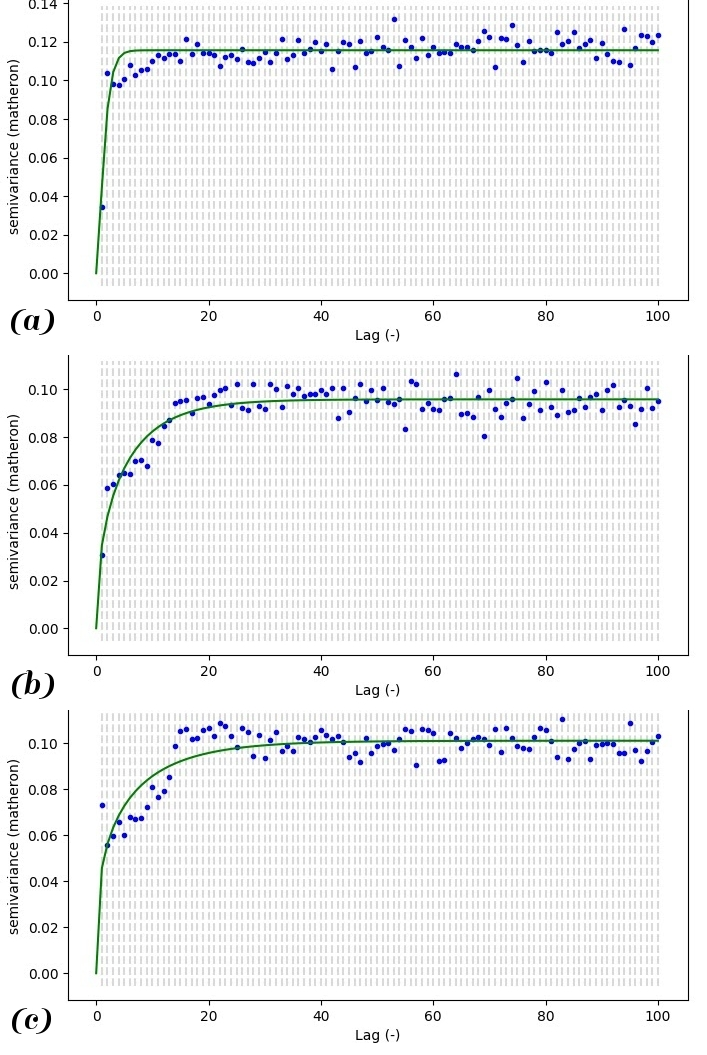
\includegraphics[width=0.58\textwidth]{fig3_allvar.jpg}
	\caption{Semivariograms for MC TBR data with coolant materials: (a) \ce{He},
	(b) \ce{H2O}, (c) \ce{D2O}}
    \label{fig:var}
  \end{center}
  \vspace{-50pt}
\end{wrapfigure}

\subsubsection{Variogram Computations}

% TODO: in results, we feature both Kriging and GPR with differing results -
% clarify their interchangeability here

Kriging is a geostatistical surrogate modelling technique which relies on correlation functions over distance (lag) in the paramater space \cite{Bouhlel2018}. Although kriging performed poorly for our use case due to high dimensionality, these correlation measures gave insight into similarities between discrete-parameter slices of the data.

\Cref{fig:var} shows the Matheron semivariance \cite{Matheron1963} for three discrete slices with coolant material varied, but all other discrete parameters fixed. Fits \cite{KrigingFig} to the Matérn covariance model confirmed numerically that the coolant material is the discrete parameter with the greatest distinguishability in the MC TBR model. 


\subsubsection{Autoencoders}

\begin{wrapfigure}{r}{0.25\textwidth}
	\centering
	\vspace{-5ex}
	{\footnotesize \incfigscale{0.8}{autoencoder}}
	\caption{Autoencoder with input width~$W_0$ and bottleneck width~$W_1$.}
	\label{fig:autoencoder}
	\vspace{-9ex}
\end{wrapfigure}

Autoencoders~\cite{SCHMIDHUBER201585} are a family of approaches to feature extraction driven by neural
networks. Faced with many possible alternatives, we implemented a conventional
autoencoder, which relies on a three-layer network that is trained to replicate
the identity mapping. While it follows that the input and output layers of such
network are sized to accommodate the analysed dataset, the
hidden layer, also called the bottleneck, allows for variable number of
neurons that represent a smaller subspace. By scanning
over a range of bottleneck widths and investigating relative changes in the
validation loss, we assess the potential for dimensional reduction.

In particular, we consider two equally-sized sets\footnote{Each set contained
\num{100000}~samples from batches 0-99 of the corresponding runs.} of samples: (i) a subset of data obtained
from run~1 and (ii) a subset of a single slice obtained from run~2. Our
expectation was that while the former case would provide meaningful insights into
correlations within the feature space, the latter would validate our
autoencoder implementation by analysing a set of points that are trivially
reducible due to a number of fixed discrete features.

\begin{wrapfigure}{l}{0.4\textwidth} % TODO: regenerate both plots as described
	\centering
	\vspace{-1ex}
	\begin{subfigure}[b]{\linewidth}
		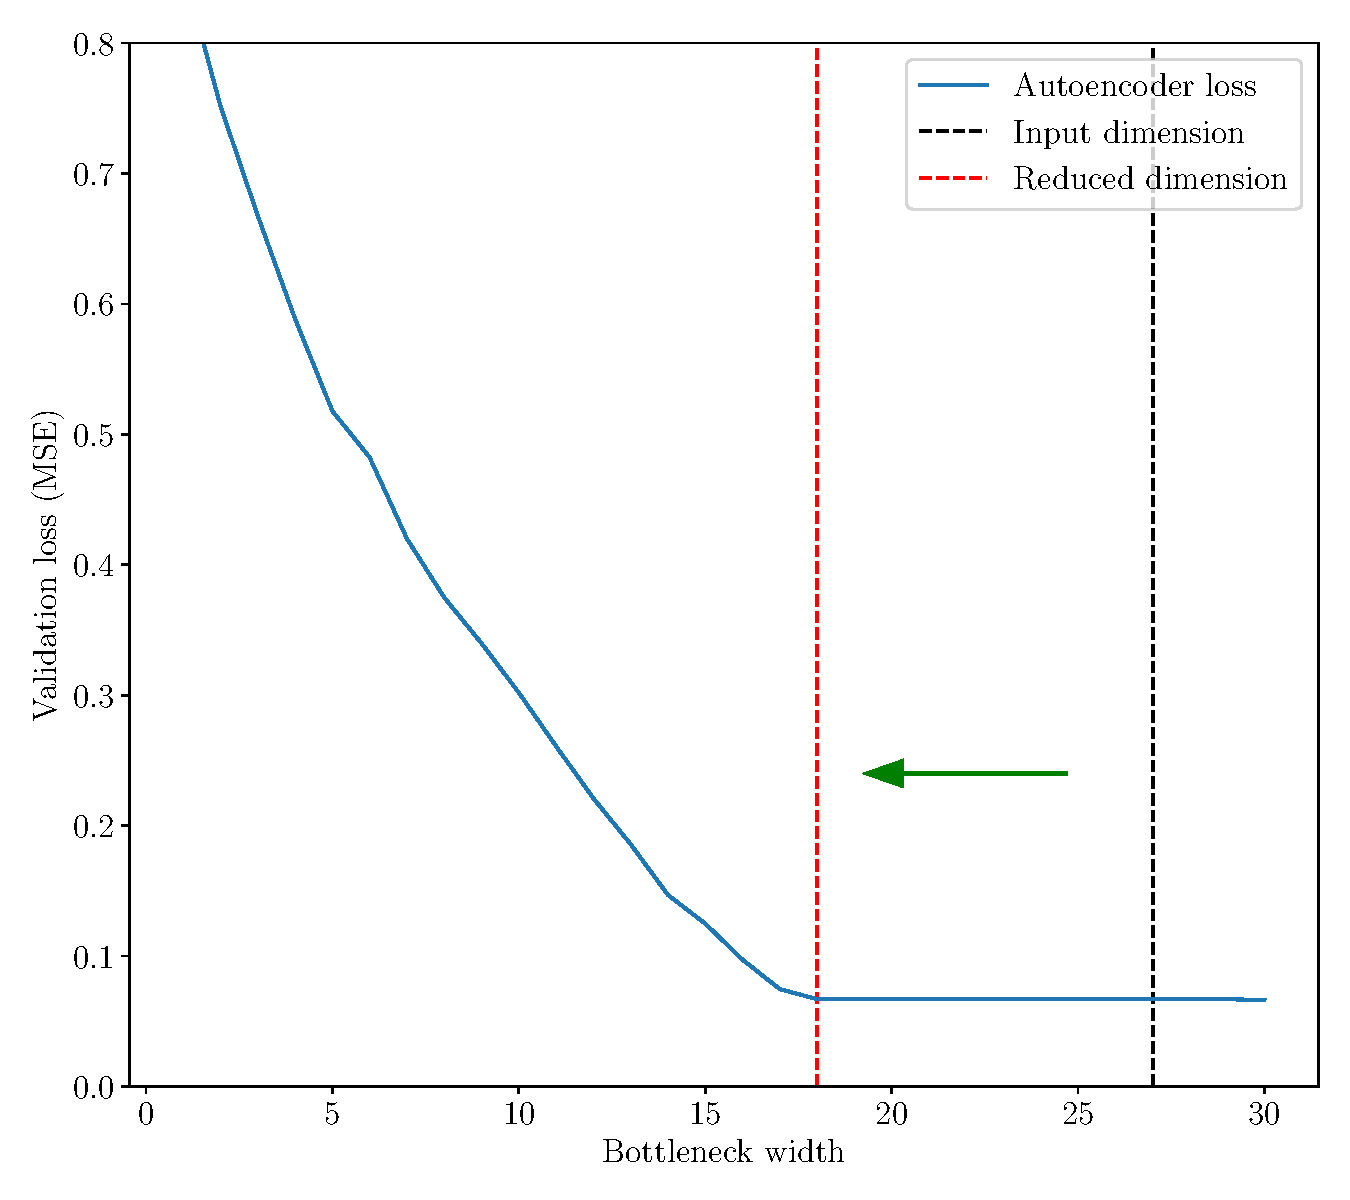
\includegraphics[width=\linewidth,trim={0 48px 0 0},clip]{ae_mixed}
	\end{subfigure}

	\vspace{-0.2ex}

	\begin{subfigure}[b]{\linewidth}
		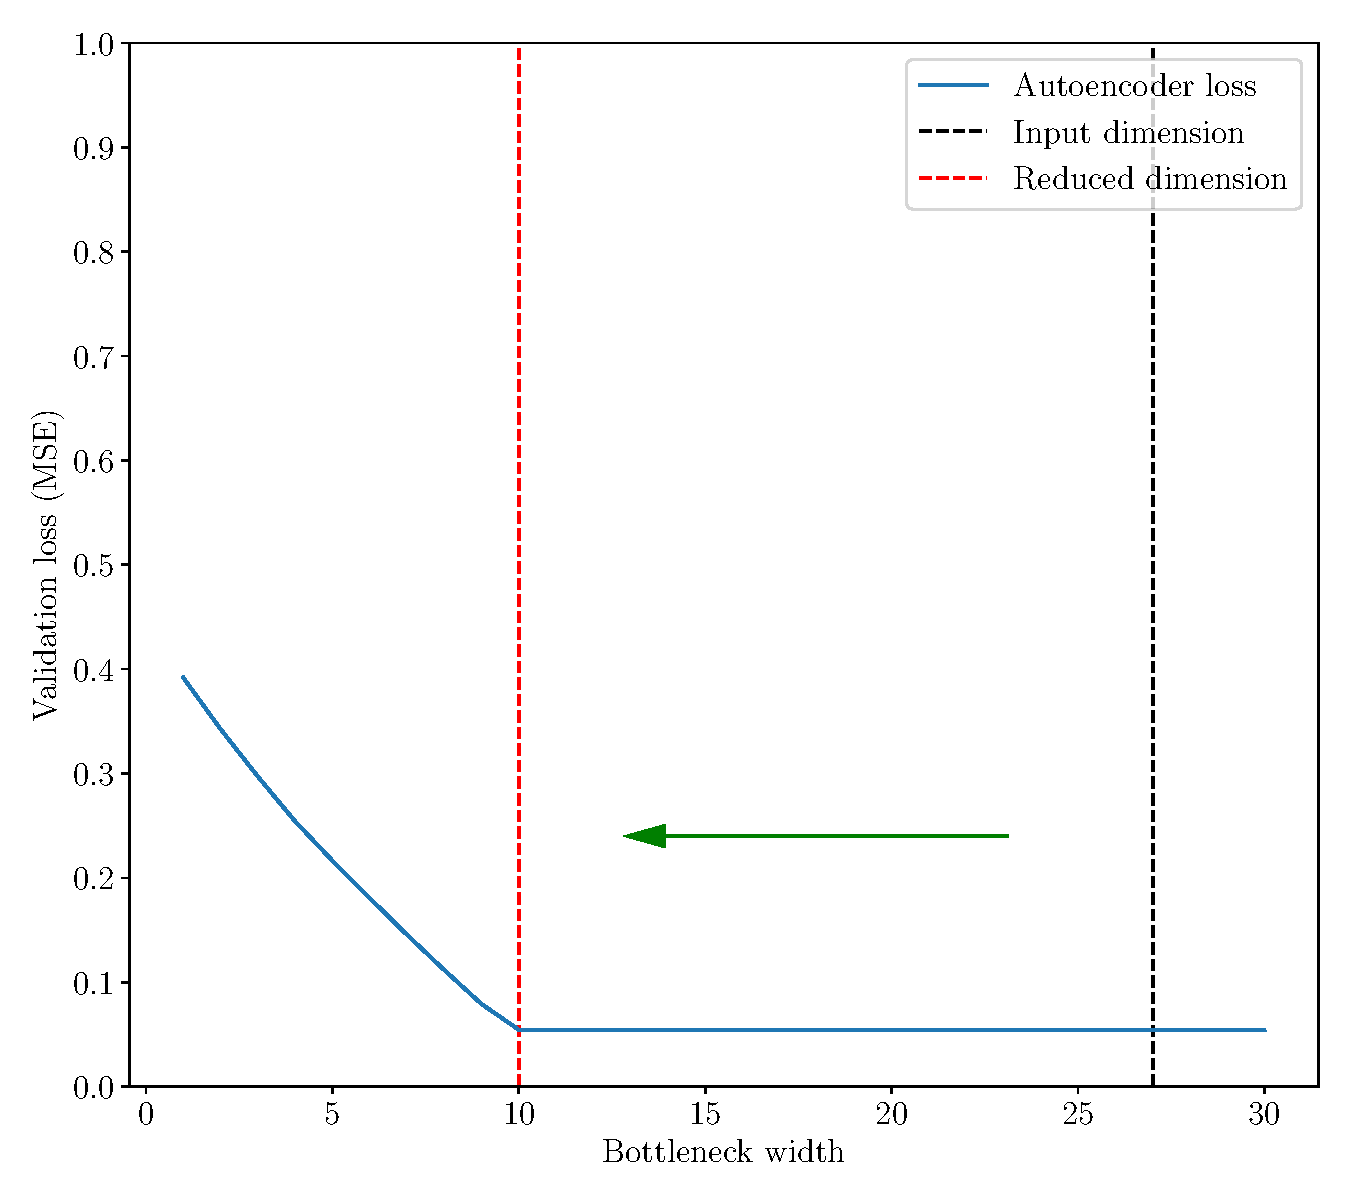
\includegraphics[width=\linewidth]{ae_single_slice}
	\end{subfigure}

	\caption{Autoencoder loss scan on the full feature space (top) and a single slice
		(bottom). Dimensional reduction is indicated by a green arrow.}
	\label{fig:autoencoder-loss}
	\vspace{-6ex}
\end{wrapfigure}

The results of both experiments are shown in~\cref{fig:autoencoder-loss}.
Consistent with our motivation, in each plot we can clearly identify a constant
plateau of low error in the region of large dimensionality followed by a point,
from which a steep increase is observed.
We consider this \textit{critical point} to mark the largest viable
dimensional reduction without significant information loss.
With this approach we find that the autoencoder was able to reduce the
datasets into a subspace of 18~dimensions in the first case and 10~dimensions in
the second case.

Confirming our expectation that in the latter, trivially reducible case the
autoencoder should achieve greater dimensional reduction, we are inclined to
believe that our implementation is indeed operating as intended. However, we
must also conclude that in both examined cases this method failed to produce a
reduction that would be superior to a naïve approach.\footnote{In both tested cases we
	can trivially eliminate 7~dimensions due to overdetermined one-hot-encoded
	features and 2~dimensions due to sum-to-one constraints. Furthermore, in the
	single slice case we may omit 7~additional dimensions due to artificially fixed
features.} This is consistent with previous results obtained by PCA and kriging.


% TODO: Question: is it accurate to say this represents nonlinear feature extraction? re my intro paragraph

